\section{Sensitivity Analysis}

An important aspect of any fuel cycle transition scenario
is the accrual of fissile materials for new reactor deployment.
The collaborative strategy makes a transition possible 
from the perspective of material availability,
but the aggressive transition demands a significant increase in reprocessing capacity.

We varied two parameters, the lifetime of French \glspl{LWR} and the
breeding ratio of \gls{ASTRID} reactors. The range over which we varies these parameters (\cref{tab:sen_par})
sought to capture the full span of their uncertainty.

\begin{table}[h]
    \centering
    \begin{tabularx}{\textwidth}{lbb}
        \hline
        \textbf{Parameter} & \textbf{Default} & \textbf{Values} \\
        \hline
        Lifetime of French \glspl{LWR} [years] & 60  & 65, 70, 80 \\
        Breeding Ratio of \glspl{ASTRID} & 1.08 & 1.11, 1.15, 1.18 \\ 
        \hline
    \end{tabularx}
    \caption {Two parameters were varied for the sensitivity analysis - the 
              lifetime of French \glspl{LWR} and the breeding ratio of \glspl{ASTRID}.
              The parameters are increased to analyze their impact on the reprocessing
              demand for the transition.}
    \label{tab:sen_par}
\end{table}

\subsection{Breeding Ratio}

Increase in the breeding ratio of \gls{ASTRID} reactors
decreases the monthly average reprocessing up to five percent,
as shown in \cref{fig:br_rep}.
However, average \gls{UOX} reprocessing demand shows little change,
because the time that reprocessed \gls{UOX} is required decrease with
increase in breeding ratio. 

\begin{figure}[htbp!]
    \begin{center}
        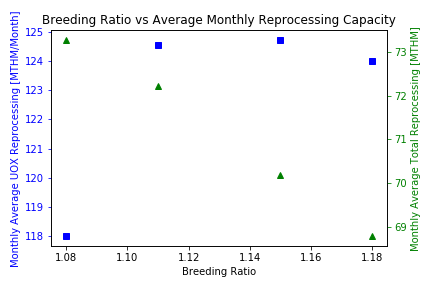
\includegraphics[scale=0.6]{./images/sensitivity/br.png}
    \end{center}
    \caption{Increasing the breeding ratio decreases the average monthly reprocessing demand for all fuels,
             but the average monthly \gls{UOX} reprocessing does not decrease due to a decrease in the time reprocess \gls{UOX} is needed. }
    \label{fig:br_rep}
\end{figure}


\begin{figure}[htbp!]
    \begin{center}
        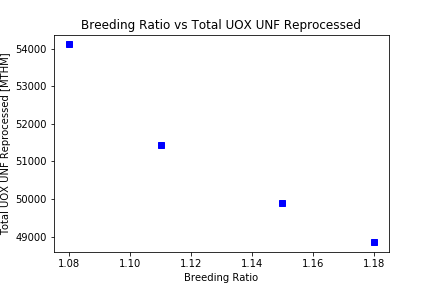
\includegraphics[scale=0.6]{./images/sensitivity/br_uox.png}
    \end{center}
    \caption{Increasing the breeding ratio decreases the number of total \gls{UOX} \gls{UNF}
             required. The \glspl{ASTRID} produce more plutonium, reducing the plutonium influx
             from reprocessed \gls{UOX}.}
    \label{fig:eu_tail}
\end{figure}


\subsection{Lifetime Extension of French \glspl{LWR}}
Extending the lifetime of French \glspl{LWR} dramatically lowers the average
monthly \gls{UOX} reprocessing demand, since the \gls{ASTRID} deployment becomes less
aggressive. The plutonium demand is delayed allowing the reprocessing plant more
time to produce plutonium for \gls{ASTRID} reactors. The
extended deployment schemes are illustrated in figure \ref{fig:ext}. 

\begin{figure}[htbp!]
    \begin{center}
        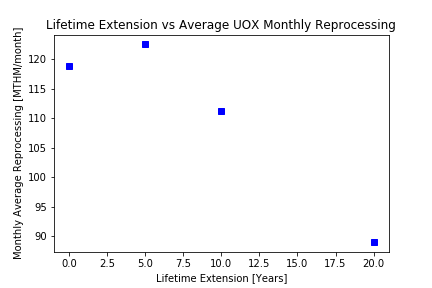
\includegraphics[scale=0.6]{./images/sensitivity/ext_uox.png}
    \end{center}
    \caption{Increasing the lifetime of French \glspl{LWR} decreases the monthly
             average \gls{UOX} reprocessing demand.}
    \label{fig:ext}
\end{figure}


\begin{figure}[htbp!]
    \begin{center}
        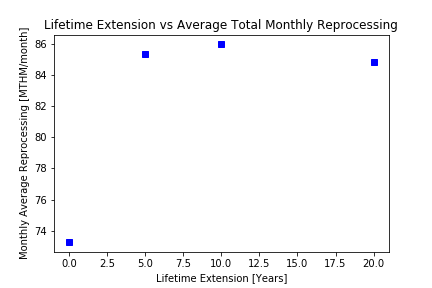
\includegraphics[scale=0.6]{./images/sensitivity/ext_all.png}
    \end{center}
    \caption{Increasing the lifetime of French \glspl{LWR} has little impact on the total monthly
             reprocessing demand.}
    \label{fig:ext}
\end{figure}


\begin{figure}[htbp!]
    \begin{center}
        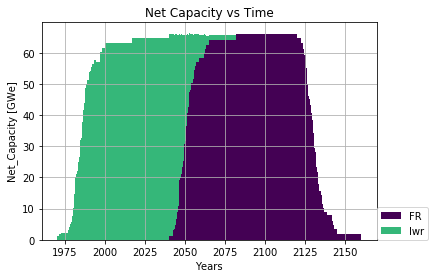
\includegraphics[height=0.25\textheight]{./images/sensitivity/5.png}
        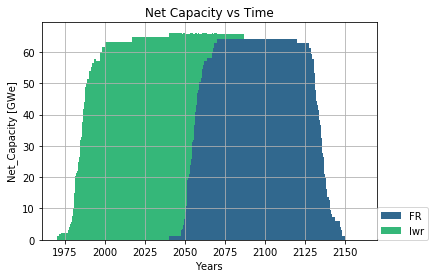
\includegraphics[height=0.25\textheight]{./images/sensitivity/10.png}
        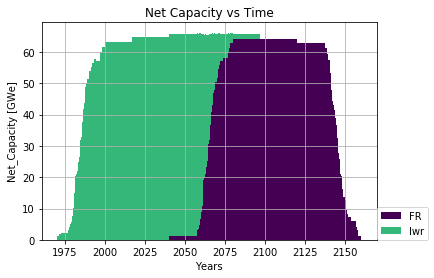
\includegraphics[height=0.25\textheight]{./images/sensitivity/20.png}
    \end{center}
    \caption{The shift in \gls{ASTRID} deployment allows more time for the reprocessing
             plant to prepare the plutonium for \gls{ASTRID} fuel production, lowering
             the average monthly reprocessing capacity.}
    \label{fig:ext}
\end{figure}


The lifetime extension of French \glspl{LWR} has little impact on the total
monthly reprocessing capacity, since the amount of plutonium in the \gls{ASTRID} used fuel
remains the same.
